% CPEN 442 -- Assignment 1 answer template (optional).
% Fill in your name(s) and answers below, compile, and submit the PDF as a1.pdf.
% You do not have to use LaTeX: any readable PDF is fine.
\documentclass[12pt]{article}

\usepackage[margin=1in]{geometry}
\usepackage[dvipsnames,table]{xcolor}
\usepackage[most]{tcolorbox}
\usepackage[hidelinks]{hyperref}
\usepackage{listings}
\usepackage{graphicx}
\usepackage{amsmath}
\usepackage{tabularx}
\usepackage{seqsplit}
\usepackage[T1]{fontenc}

\definecolor{aliceblue}{rgb}{0.7, 1, 1}
\definecolor{background}{rgb}{1, 0.98, 0.95}

\lstset{frame=tb, language=Python, showstringspaces=false, columns=flexible,
  basicstyle={\small\ttfamily}, breaklines=true, backgroundcolor=\color{background}}

\setlength{\parindent}{0in}
\setlength{\parskip}{\baselineskip}

\newcounter{question}
\newcommand{\question}[1]{\refstepcounter{question}%
  \textbf{\colorbox{aliceblue}{[#1 pts]} Question \arabic{question}}}

% Box to write each answer in. It grows with its content.
\newtcolorbox{answer}{colback=white, colframe=black, boxrule=0.4pt,
  sharp corners, breakable}

\begin{document}

\begin{center}
    THE UNIVERSITY OF BRITISH COLUMBIA\\
    Electrical and Computer Engineering Department\\[\baselineskip]
    {\bf CPEN 442\hfill Introduction to Cybersecurity\hfill Winter Term 1, 2026}
    \vspace{1cm}

    {\sc \Large Assignment 1: Ancient Crypto}
\end{center}

% One or two students. Delete the second row if you worked alone.
\begin{tabularx}{\textwidth}{|X|l|}
    \hline
    \rowcolor{gray!15} \textbf{Name} & \textbf{Student number} \\
    \hline
    Chongkai (Lucas) Lyu & 30349559 \\
    \hline
    Leyang Gao & 58256207 \\
    \hline
\end{tabularx}

\textbf{Canvas assignment group number:} ?

\section{The Index of Coincidence (IC)}

\question{20} For each of Caesar, affine, Vigen{\`e}re, and Playfair, is the IC of the ciphertext expected to be higher, lower, or equal to the plaintext's IC? Explain why.

\begin{answer}
    \textbf{Caesar:} equal

    \textbf{Explanation:}
    Caesar cipher shifts every letter by a fixed number. Since each plaintext letter is mapped to exactly one ciphertext letter, the letter frequencies remain unchanged, and therefore the IC stays the same.

    \bigskip
    \textbf{Affine:} equal

    \textbf{Explanation:}
    Affine cipher uses a one-to-one substitution, mapping each plaintext letter to a unique ciphertext letter. This preserves the letter frequency distribution, so the IC remains unchanged. This mapping is a permutation of the alphabet.

    \bigskip
    \textbf{Vigen{\`e}re:} lower

    \textbf{Explanation:}
    Vigen{\`e}re cipher uses different shifts depending on the position of the letter in the repeating key. Therefore, the same plaintext letter can be encrypted into different ciphertext letters, making the letter frequency distribution more uniform and generally reducing the IC. If the key length is 1, Vigen{\`e}re reduces to Caesar and the IC is unchanged.

    \bigskip
    \textbf{Playfair:} lower

    \textbf{Explanation:}
    Playfair cipher encrypts pairs of letters rather than individual letters. The encryption of each letter depends on the other letter in its pair. This disrupts the original single-letter frequency distribution, making it generally more uniform and reducing the expected IC.
\end{answer}

\clearpage
\section{Detecting Ciphers}

\question{30} Without breaking them, which line of \texttt{ciphertexts\_$i$.txt} corresponds to which cipher? Explain how you figured out each one.

\begin{answer}
    The six lines of \texttt{ciphertexts\_80.txt}:

    \begingroup
    \setlength{\parindent}{0pt}%
    \setlength{\parskip}{0pt}%
    \scriptsize\ttfamily
    \noindent 1)\ \seqsplit{PRWAKPWAGBQYBHDWPSNQPOWKOZZQYCINQDQMAHFZMQMUZPDPIUMQLFNBRLONCSYCHUQBRLPGBOGPRGDPTVQWHABAGPWQBQHVHVMGKFRGXPKMGPHUVYLMLFSMBNKFHVVUMQTDPSYCWBUMKXKFZNQZRXHWCLBWHRQDVUMFTQKLDPVCDFOBUIBQGCXHBQSRESMYOMUKDPYPDPTVDPNUXQQBBEHPONFZOZKOZNQLONCHWKOLUZGPYVBUMQHKONVSVURXPVCSFUVUMQTDPSDPZAOGUMMQHTBOHGHDXKNVGPHTMQMU}\par
    \vspace{\baselineskip}
    \noindent 2)\ \seqsplit{GZCKPFCSAPCRWSGHFOBGWHWCBOBRAOHIFWHMKWHVWHGQOZARSASOBCFOBRSJCZJWBUOPWZWHWSGWHRSACBGHFOHSGHVOHUFCKHVFSEIWFSGPCHVORODHOHWCBOBROQQSDHOBQSGZCKPFCHSOQVSGHVOHQVOBUSQOBPFWBUBSKGHFSBUHVGWHFSTZSQHGHVSWADCFHOBQSCTDOHWSBQSOBRHWAWBUGVCKWBUHVOHHFISRSJSZCDASBHPOZOBQSGQCBHWBIWHMKWHVHFOBGTCFAOHWCB}\par
    \vspace{\baselineskip}
    \noindent 3)\ \seqsplit{B3P3R6IFG5Q7SOUUMDKFFFMPZ2SKKXHYT2F6DZB2EFSXDTI3WEI542Q4X4UYYPVMIDOZW4MBXXDUGNGNEILQLXNMADQQ55YIQT3JD5Y4QOLOPJRMIS3OCV2YENQFMJP4IAJINJIJP7LYM2RWQIKZEZL4K7PFVYJOS7EVWQ6AL4T6B34HHJ2OC7PFTNCBHSQL4VYPBIMGYKZ6RK3BEMXP5T2ZAWBTTJKOAKBWFNUCCGHG7YOFBTVJT5H4FA76JU5TPZM4XP24GAFLQUANIWGV7CCLTSO2LIQAL2PIBGSOWIWKYKQCHYZLE2}\par
    \vspace{\baselineskip}
    \noindent 4)\ \seqsplit{F6ADXSKGN5QCHHVCOUJ4PIIVKPQDJYKIOUQS34SWWXS3ISIO3MIEXSQZ2JYDNAV6XVOZWAM6HNQFCTQMXVR65RRRLRVT3UHN4P2JD7VTABKYDLHA7YK5DIEND3DHGO6L2OJCEEBTPS6YKVD4RWCTMVH7DNYDXZOMCOEQHFLBMQ4OBNAARJPIPPNBEFEJUFVDA3D6X6GKSMHSC7LEPUVAJLLXRCO4SNR5KKB5OE7UTVCZAUYJFTHNZK2LFW2KJXWAFPKXU4WJRX56WKUNI}\par
    \vspace{\baselineskip}
    \noindent 5)\ \seqsplit{NFYVCLEJQDEQDJDSCJEQDRBJBLSFSKJNBGGHBCIJIFQEGBZYJFSKWLRVJDKZLCBLSBCKDZLSJCQFCDJZFJCDQTCIQLVPIEQFRCBRDFSKQDWBSDZDSCNFYVCLEJCDFRIDJCIFCRLSJBJCDSCDWWLQCFSKFKFECFYBGBCTGDFKCLDWWBRBDSRTBCQDWGDRCJKBJRBEGBSDFPBGBCTFSKJCQFCDPBRRFEFYBGBCTNFYVCLEJDZYLKBDJJNBGGQDWBSDZDSCFSKRLSCQLGGDKJCQDSPCI}\par
    \vspace{\baselineskip}
    \noindent 6)\ \seqsplit{CUGFEKEHEEBFTCEKCFBFATOIQNIGNRDXSQNVHAYXOICYDXRFCGUDTZFFEMNZJMILDVCINKTIQNEKTYUJOOEIEZCGOITCNSTZEHMSGEUNOFTVQWHWSKXUTLERCQOJKRCJLAFZUMCSPRRCLATPYNRWFCUWTKTYUCMHOIJUNUEFVWODLVSNINEVVZOJTRDXADIXDGEFTJXIWANXJBALCFCVIFEUVICMSJJLEFGKXYNKIEVFUWNTUUNVEWVYCLIMUHEKSDQANWTFDYMTOUYYSMNZJSEXFZSCEFCPQHDKTIQNEYITSIOJDZDUTAOE}\par
    \endgroup

    \bigskip
    For this question, the ciphers are identified in this order: OTP first, then Playfair, then Vigen{\`e}re, then Caesar, and finally Affine.

    These two figures are the letter-frequency plots of the remaining lines, line 2 and line 5.

    \begin{center}
        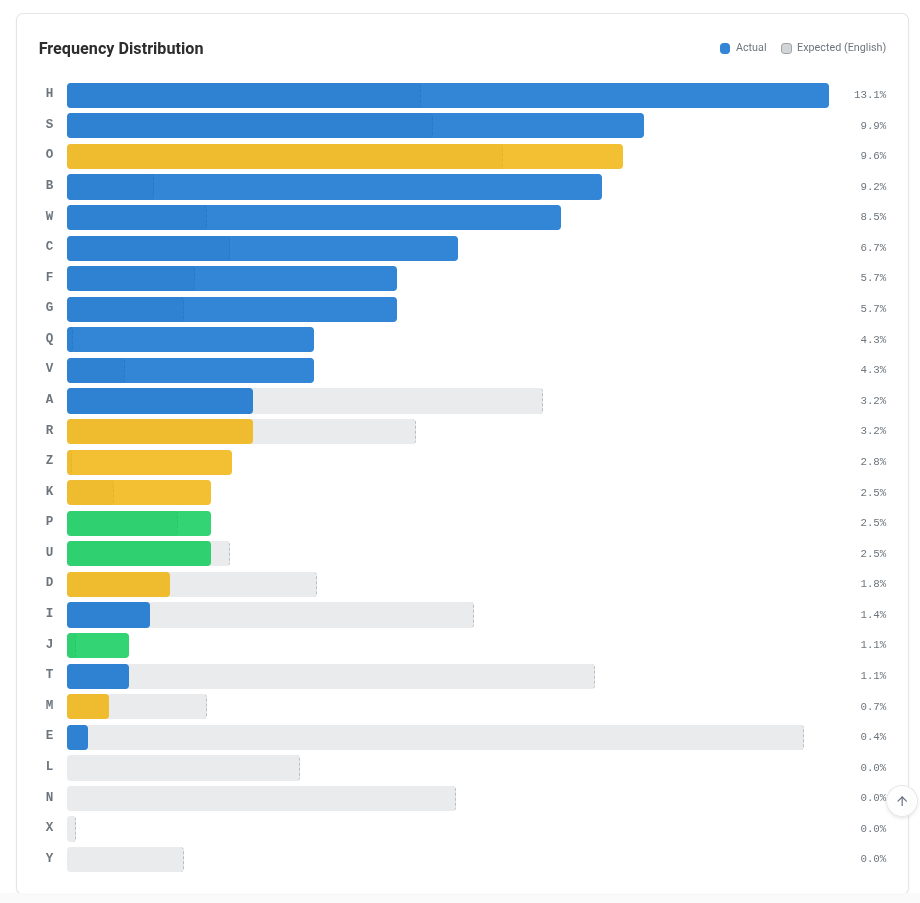
\includegraphics[width=\linewidth]{cipher2_frequency.png}

        \smallskip
        Line 2. The ciphertext was pasted into {\hypersetup{pdfborder={0 0 0}}\url{https://caesarcipher.org/ciphers/frequency-analysis}}, which drew this chart.
    \end{center}

    \begin{center}
        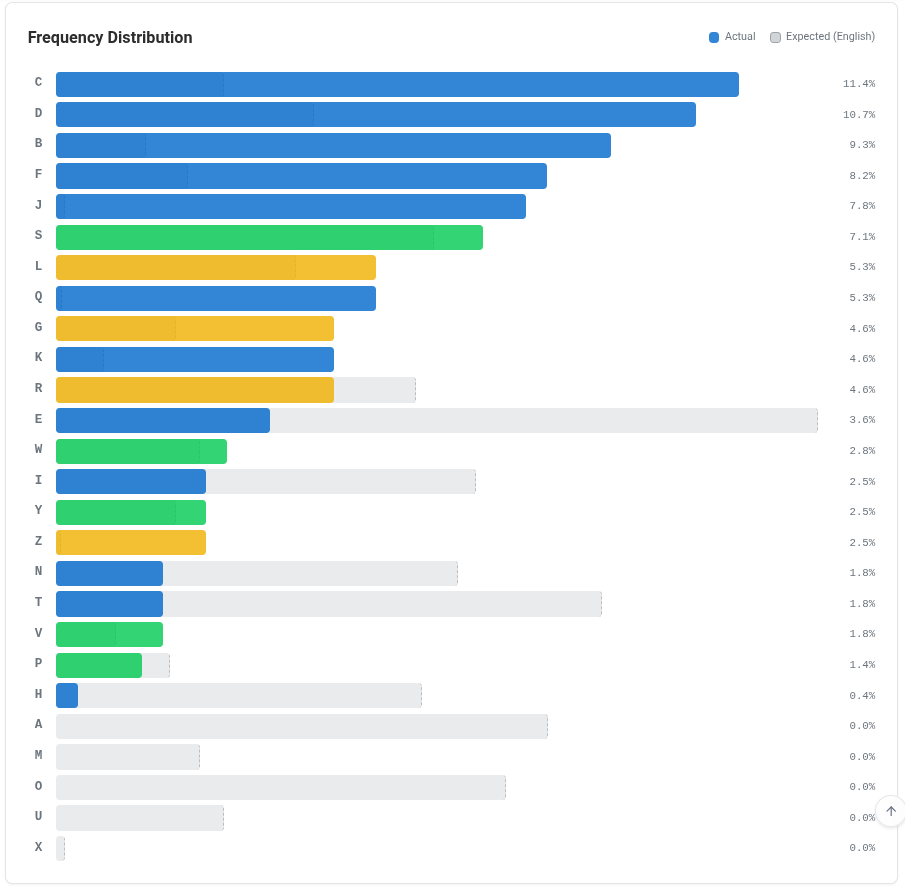
\includegraphics[width=\linewidth]{cipher5_frequency.png}

        \smallskip
        Line 5. Same tool, {\hypersetup{pdfborder={0 0 0}}\url{https://caesarcipher.org/ciphers/frequency-analysis}}.
    \end{center}

    \bigskip
    \textbf{Caesar:} line 2

    \textbf{Explanation:}
    Caesar shifts every letter by the same $x$. Guess which bar is E; then T, A, O, \ldots\ are that letter plus the same $x$. A red cell is under 1\%, so that guess is wrong.

    \textbf{Line 2.}
    $\mathrm{E}\to\mathrm{H}$ ($x=3$) sends I to L (0\%), so it is wrong. $\mathrm{E}\to\mathrm{S}$ ($x=14$) keeps E through D high, so line 2 is Caesar with shift 14.

    \begin{center}
    \resizebox{\linewidth}{!}{%
    \begin{tabular}{l r c c c c c c c c c c}
    \hline
    Image of E & $x$ & E & T & A & O & I & N & S & H & R & D \\
    \hline
    H (13.1\%) & 3 & H 13.1\% & W 8.5\% & D 1.8\% & R 3.2\% & \textcolor{red}{L 0.0\%} & Q 4.3\% & V 4.3\% & K 2.5\% & U 2.5\% & G 5.7\% \\
    S (9.9\%) & 14 & S 9.9\% & H 13.1\% & O 9.6\% & C 6.7\% & W 8.5\% & B 9.2\% & G 5.7\% & V 4.3\% & F 5.7\% & R 3.2\% \\
    \hline
    \end{tabular}}
    \end{center}

    \medskip
    \textbf{Line 5.}
    Every row has a red cell, so no single shift fits. Line 5 is not Caesar.

    \begin{center}
    \resizebox{\linewidth}{!}{%
    \begin{tabular}{l r c c c c c c c c c c}
    \hline
    Image of E & $x$ & E & T & A & O & I & N & S & H & R & D \\
    \hline
    C (11.4\%) & 24 & C 11.4\% & R 4.6\% & Y 2.5\% & \textcolor{red}{M 0.0\%} & G 4.6\% & L 5.3\% & Q 5.3\% & F 8.2\% & P 1.4\% & B 9.3\% \\
    D (10.7\%) & 25 & D 10.7\% & S 7.1\% & Z 2.5\% & N 1.8\% & \textcolor{red}{H 0.4\%} & M 0.0\% & R 4.6\% & G 4.6\% & Q 5.3\% & C 11.4\% \\
    B (9.3\%) & 23 & B 9.3\% & Q 5.3\% & \textcolor{red}{X 0.0\%} & L 5.3\% & F 8.2\% & K 4.6\% & P 1.4\% & E 3.6\% & O 0.0\% & A 0.0\% \\
    F (8.2\%) & 1 & F 8.2\% & \textcolor{red}{U 0.0\%} & B 9.3\% & P 1.4\% & J 7.8\% & O 0.0\% & T 1.8\% & I 2.5\% & S 7.1\% & E 3.6\% \\
    J (7.8\%) & 5 & J 7.8\% & Y 2.5\% & F 8.2\% & T 1.8\% & N 1.8\% & S 7.1\% & \textcolor{red}{X 0.0\%} & M 0.0\% & W 2.8\% & I 2.5\% \\
    S (7.1\%) & 14 & S 7.1\% & \textcolor{red}{H 0.4\%} & O 0.0\% & C 11.4\% & W 2.8\% & B 9.3\% & G 4.6\% & V 1.8\% & F 8.2\% & R 4.6\% \\
    L (5.3\%) & 7 & L 5.3\% & \textcolor{red}{A 0.0\%} & H 0.4\% & V 1.8\% & P 1.4\% & U 0.0\% & Z 2.5\% & O 0.0\% & Y 2.5\% & K 4.6\% \\
    Q (5.3\%) & 12 & Q 5.3\% & F 8.2\% & \textcolor{red}{M 0.0\%} & A 0.0\% & U 0.0\% & Z 2.5\% & E 3.6\% & T 1.8\% & D 10.7\% & P 1.4\% \\
    G (4.6\%) & 2 & G 4.6\% & V 1.8\% & C 11.4\% & Q 5.3\% & K 4.6\% & P 1.4\% & \textcolor{red}{U 0.0\%} & J 7.8\% & T 1.8\% & F 8.2\% \\
    K (4.6\%) & 6 & K 4.6\% & Z 2.5\% & G 4.6\% & \textcolor{red}{U 0.0\%} & O 0.0\% & T 1.8\% & Y 2.5\% & N 1.8\% & X 0.0\% & J 7.8\% \\
    R (4.6\%) & 13 & R 4.6\% & G 4.6\% & N 1.8\% & B 9.3\% & V 1.8\% & \textcolor{red}{A 0.0\%} & F 8.2\% & U 0.0\% & E 3.6\% & Q 5.3\% \\
    \hline
    \end{tabular}}
    \end{center}

    \bigskip
    \textbf{Affine:} line 5

    \textbf{Explanation:}
    Line 5 is the other monoalphabetic line, and the table shows it is not a fixed shift, so it is Affine.

    \bigskip
    \textbf{Vigen{\`e}re:} line 6

    \textbf{Explanation:}
    After identifying Playfair (line 1) and OTP (lines 3 and 4), the remaining candidates are lines 2, 5, and 6. Caesar and Affine are monoalphabetic, so their IC should stay close to English. Vigen{\`e}re is polyalphabetic, so its IC should drop toward a random string.

    \textbf{Steps.}
    \begin{enumerate}
        \item Compute the unnormalized IC
        \[
        \kappa=\sum_{i}\frac{n_i(n_i-1)}{N(N-1)}.
        \]
        \item Multiply by 26 so the values can be compared with the figures on Wikipedia ({\hypersetup{pdfborder={0 0 0}}\url{https://en.wikipedia.org/wiki/Index_of_coincidence}}): English $\approx 1.73$, uniform random $= 1.00$.
        \item Results for the three remaining lines:
        \begin{itemize}
            \item Line 2: $0.06878\times 26=1.79$
            \item Line 5: $0.06472\times 26=1.68$
            \item Line 6: $0.04308\times 26=1.12$
        \end{itemize}
        \item Lines 2 and 5 are both near $1.73$, so they are Caesar or Affine. Line 6 differs most from $1.73$ and is closest to $1.00$, therefore it is Vigen{\`e}re.
    \end{enumerate}

    \bigskip
    \textbf{Playfair:} line 1

    \textbf{Explanation:}
    Line 1 is the only ciphertext that contains no letter J. In this assignment, Playfair replaces every J with I and uses a 25-letter key that excludes J, so a Playfair ciphertext can never contain J. The other letter-only lines (2, 5, and 6) all contain J, so they cannot be Playfair.

    \bigskip
    \textbf{OTP:} lines 3, 4

    \textbf{Explanation:}
    Lines 3 and 4 are the only ciphertexts that contain digits. The OTP in this assignment encodes letters as 5-bit symbols with the RFC 4648 Base32 alphabet (A--Z and 2--7), XORs them with the pad, and encodes the result back with the same alphabet. Therefore an OTP ciphertext can include the digits 2--7, whereas Caesar, Affine, Vigen{\`e}re, and Playfair output only A--Z. This also matches the note that OTP was used twice.
\end{answer}

\section{Breaking Ciphers}

\question{50} For each ciphertext, give the name of the Pok{\'e}mon described in the plaintext and explain how you found it.

\begin{answer}
    % Leave a name as "?" if you could not break that cipher.
    \textbf{Caesar:} Slowbro

    \textbf{Explanation:}
    Question 2 gave the key \(x = 14\). Subtract 14 from every letter. The plaintext begins with SLOWBRO.

    \smallskip
    {\scriptsize\ttfamily\seqsplit{SLOWBROEMBODIESTRANSITIONANDMATURITYWITHITSCALMDEMEANORANDEVOLVINGABILITIESITDEMONSTRATESTHATGROWTHREQUIRESBOTHADAPTATIONANDACCEPTANCESLOWBROTEACHESTHATCHANGECANBRINGNEWSTRENGTHSITREFLECTSTHEIMPORTANCEOFPATIENCEANDTIMINGSHOWINGTHATTRUEDEVELOPMENTBALANCESCONTINUITYWITHTRANSFORMATION}}

    \bigskip
    \textbf{Affine:} Kabutops

    \textbf{Explanation:}
    Encryption is \(ax+b\equiv y\pmod{26}\), so \(ax\equiv y-b\pmod{26}\). Decryption needs \(a^{-1}\), and that exists only when \(\gcd(a,26)=1\). The 12 possible values of \(a\) are
    \[
    1,3,5,7,9,11,15,17,19,21,23,25.
    \]
    The tallest ciphertext bars are C, D, B, F, and the common English letters are E, T, A, O. Pair them and solve. \(\mathrm{E}\to\mathrm{D}\) and \(\mathrm{T}\to\mathrm{C}\) give
    \begin{align*}
    4a+b &\equiv 3 \pmod{26},\\
    19a+b &\equiv 2 \pmod{26}.
    \end{align*}
    Subtract: \(15a\equiv 25\pmod{26}\). Since \(15\cdot 7\equiv 1\), \(a\equiv 25\cdot 7\equiv 19\). Then \(4\cdot 19+b\equiv 3\), so \(b\equiv 5\).

    With \(a=19\) and \(b=5\), the encryption formula is
    \[
    19x\equiv y-5\pmod{26}.
    \]
    Multiply both sides by a number \(k\):
    \[
    19kx\equiv k(y-5)\pmod{26}.
    \]
    The left side should be only \(x\), so \(k\) must satisfy \(19k\equiv 1\pmod{26}\). Then
    \[
    19kx\equiv 1\cdot x\equiv x\pmod{26}.
    \]
    \(19\cdot 11=209=8\cdot 26+1\), so \(k=11\). Each ciphertext letter \(y\) becomes \(11(y-5)\bmod 26\). The plaintext begins with KABUTOPS.

    \smallskip
    {\scriptsize\ttfamily\seqsplit{KABUTOPSREPRESENTSPRECISIONANDSKILLWITHSHARPLIMBSANDFOCUSEDMOTIONITDEMONSTRATESMASTERYTHROUGHPRACTICEANDREFINEMENTKABUTOPSTEACHESTHATCONSISTENTEFFORTANDADAPTABILITYLEADTOEFFICIENCYITREFLECTSDISCIPLINEAGILITYANDSTRATEGICCAPABILITYKABUTOPSEMBODIESSKILLREFINEMENTANDCONTROLLEDSTRENGTH}}

    \bigskip
    \textbf{Vigen{\`e}re:} Magneton

    \textbf{Explanation:}
    Line 6 has 312 letters. Its IC is \(1.120\), near a random string. For a guessed key length \(k\), group \(i\) is letters \(i, i+k, i+2k, \ldots\). Those letters share one key letter, so a correct \(k\) makes each group's IC near English, about \(1.73\). The groups below start at \(k=3\).

    \textbf{Key length 3.} 104 letters each.
    \begin{quote}\scriptsize\ttfamily
    1.\ \seqsplit{CFEETKBTQGDQHXCXCDFMJLCKQKUOEGTSESUFQWXLCJCAUSRAYWUKUHJUVDSNVJDDDFXAJLCFVMJFXKVWUVVLUKQWDTYMJXSFQKQYSJDA}\\
    2.\ \seqsplit{UEHBCCFONNXNAOYRGTFNMDITNTJEZOCTHGNTWSUEQKJFMPCTNFWTCOUEWLNEZTXIGTINBCVEISLGYIFNUEYIHSATYOYNSFCCHTNIIDUO}\\
    3.\ \seqsplit{GKEFEFAIIRSVYIDFUZEZIVNIEYOICINZMEOVHKTRORLZCRLPRCTYMINFOVIVORAXEJWXAFIUCJEKNEUTNWCMEDNFMUSZEZEPDIETOZTE}
    \end{quote}

    \textbf{Key length 4.} 78 letters each.
    \begin{quote}\scriptsize\ttfamily
    1.\ \seqsplit{CEETCAQNSHODCTEJDNQTOEONEGOQSTCKLUPLYFTUONVLIVTADTWJCIVSEXIUUECUSNDOSJFEQTESDT}\\
    2.\ \seqsplit{UKECFTNRQAIXGZMMVKNYOZISHEFWKLQRAMRANCKCIUWVNZRDGJABFFIJFYEWUWLHDWYUMSZFHIYIZA}\\
    3.\ \seqsplit{GEBEBOIDNYCRUFNICTEUECTTMUTHXEOCFCRTRUTMJEOSEODIEXNACECJGNVNNVIEQTMYNESCDQIODO}\\
    4.\ \seqsplit{FHFKFIGXVXYFDFZLIIKJIGCZSNVWURJJZSCPWWYHUFDNVJXXFIXLVUMLKKFTVYMKAFTYZXCPKNTJUE}
    \end{quote}

    \textbf{Key length 5.} The first two groups have 63 letters; the last three have 62.
    \begin{quote}\scriptsize\ttfamily
    1.\ \seqsplit{CKBKANDVOXUFJVTKOZTZGFHUCRFSLNUYOUONVRIFWBCUSFNFUWIKNYYZFFDNSZO}\\
    2.\ \seqsplit{UEFCTIXHIRDEMCITOCCEETWTQCZPARWUIEDIZDXTAAVVJGKUUVMSWMYJZCKEIDE}\\
    3.\ \seqsplit{GHTFOGSACFTMIIQYEGNHUVSLOJURTWTCJFLNOXDJNLIIJKIWNYUDTTSSSPTYOU}\\
    4.\ \seqsplit{FECBINQYYCZNLNNUIOSMNQKEJLMRPFKMUVVEJAGXXCFCLXENVCHQFOMECQIIJT}\\
    5.\ \seqsplit{EEEFQRNXDGFZDKEJEITSOWXRKACCYCTHNWSVTDEIJFEMEYVTELEADUNXEHQTDA}
    \end{quote}

    \textbf{Key length 6.} 52 letters each.
    \begin{quote}\scriptsize\ttfamily
    1.\ \seqsplit{CETBQDHCCFJCQUETEUQXCCURYUUJVSVDDXJCVJXVUVUQDYJSQQSD}\\
    2.\ \seqsplit{UHCFNXAYGFMINJZCHNWUQJMCNWCUWNZXGIBVILYFUYHAYYSCHNIU}\\
    3.\ \seqsplit{GEEAISYDUEINEOCNMOHTOLCLRTMNOIOAEWAICENUNCENMSEEDEOT}\\
    4.\ \seqsplit{FEKTGQXXDMLKKOGSSFWLJASAWKHUDNJDFALFMFKWVLKWTMXFKYJA}\\
    5.\ \seqsplit{EBCONNORTNDTTEOTGTSEKFPTFTOELETITNCESGINEISTONFCTIDO}\\
    6.\ \seqsplit{KFFIRVIFZZVIYIIZEVKRRZRPCYIFVVRXJXFUJKETWMDFUZZPITZE}
    \end{quote}

    The IC below is already multiplied by 26, and the reported value is the average of the \(k\) groups. Checked from \(k=3\) to \(k=20\).

    \begin{center}
    \small
    \begin{tabular}{c c l}
    \hline
    Key length & Average IC & Note \\
    \hline
    3 & 1.298 & \\
    4 & 1.279 & \\
    5 & 1.224 & \\
    \textbf{6} & \textbf{1.797} & shortest clear peak \\
    7 & 0.983 & \\
    8 & 1.351 & \\
    9 & 1.323 & \\
    10 & 1.484 & \\
    11 & 1.050 & \\
    12 & 1.727 & multiple of 6 \\
    13 & 1.138 & \\
    14 & 1.123 & \\
    15 & 1.497 & \\
    16 & 1.355 & \\
    17 & 1.031 & \\
    18 & 1.912 & multiple of 6 \\
    19 & 1.063 & \\
    20 & 1.430 & \\
    \hline
    \end{tabular}
    \end{center}

    Lengths 6, 12, and 18 peak. If the true length is 6, grouping every 12 or 18 letters still puts only one key letter in each group, so those multiples stay high. The shortest clear peak is 6.

    \medskip
    Group ICs for 3, 4, and 6:

    \begin{center}
    \small
    \begin{tabular}{c c c c c c}
    \hline
    \multicolumn{2}{c}{\(k=3\)} & \multicolumn{2}{c}{\(k=4\)} & \multicolumn{2}{c}{\(k=6\)} \\
    Group & IC & Group & IC & Group & IC \\
    \hline
    1 & 1.218 & 1 & 1.446 & 1 & 1.922 \\
    2 & 1.345 & 2 & 0.970 & 2 & 1.353 \\
    3 & 1.330 & 3 & 1.532 & 3 & 1.961 \\
      &       & 4 & 1.169 & 4 & 1.392 \\
      &       &   &       & 5 & 2.412 \\
      &       &   &       & 6 & 1.745 \\
    \hline
    avg & 1.298 & avg & 1.279 & avg & 1.797 \\
    \hline
    \end{tabular}
    \end{center}

    At length 6 every group stays near or above English. At 3 and 4 some groups stay near 1. The groups do not need identical ICs: each one is a Caesar shift of English, so the values move around 1.73. The key length is 6.

    Each group is one Caesar cipher. The frequency charts, in group order:

    \begin{center}
        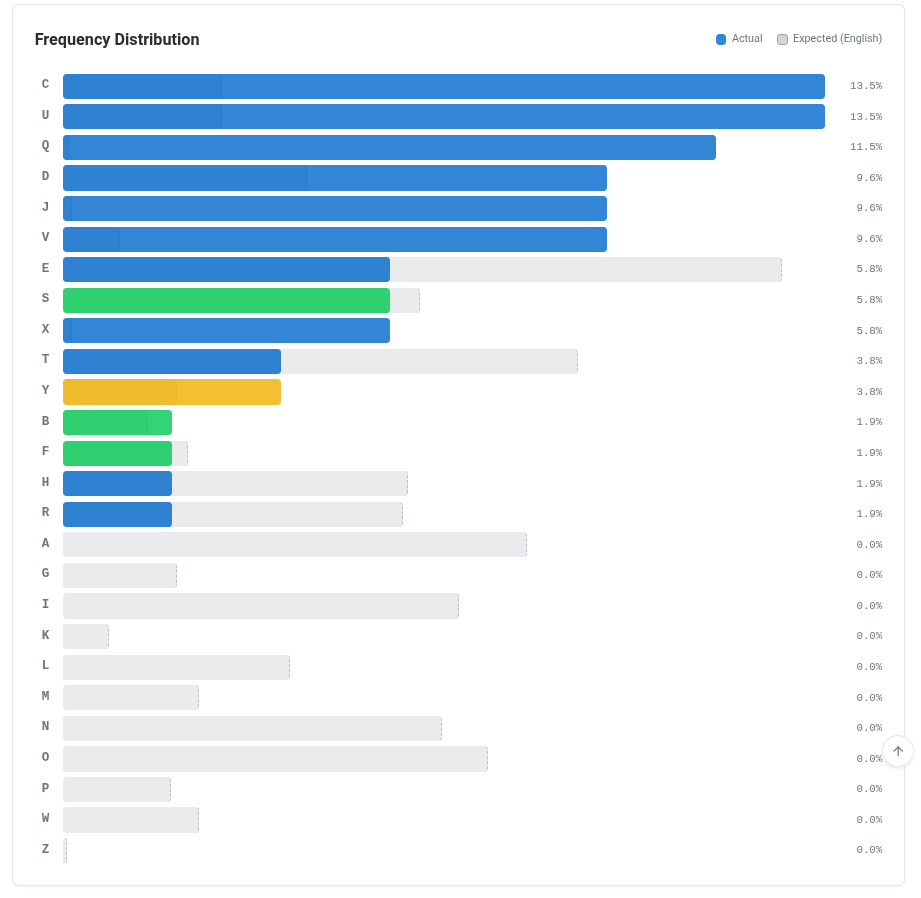
\includegraphics[width=\linewidth]{cipher6_g1_frequency.png}

        \smallskip
        Group 1
    \end{center}

    \begin{center}
        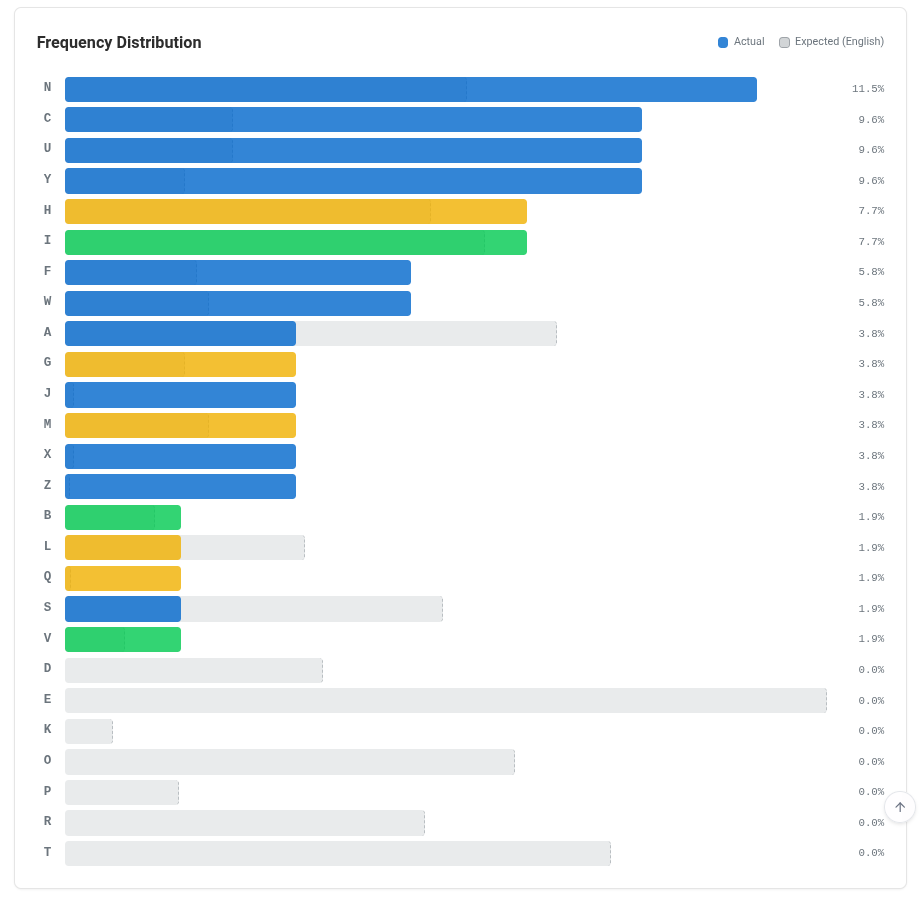
\includegraphics[width=\linewidth]{cipher6_g2_frequency.png}

        \smallskip
        Group 2
    \end{center}

    \begin{center}
        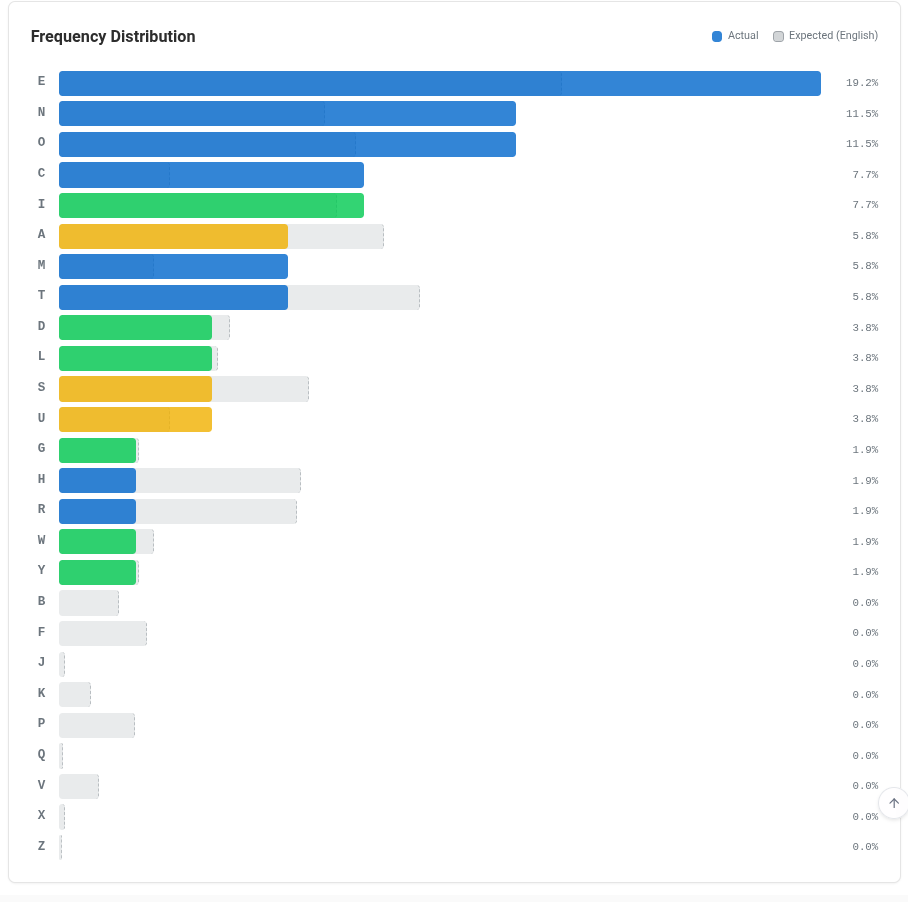
\includegraphics[width=\linewidth]{cipher6_g3_frequency.png}

        \smallskip
        Group 3
    \end{center}

    \begin{center}
        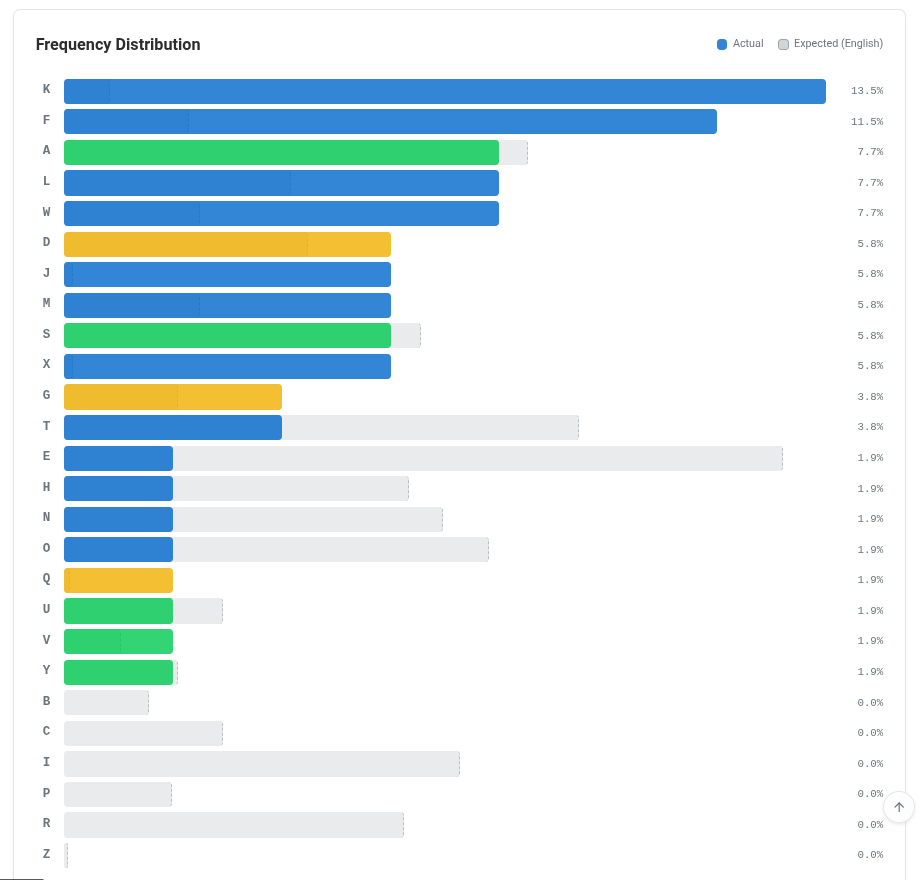
\includegraphics[width=\linewidth]{cipher6_g4_frequency.png}

        \smallskip
        Group 4
    \end{center}

    \begin{center}
        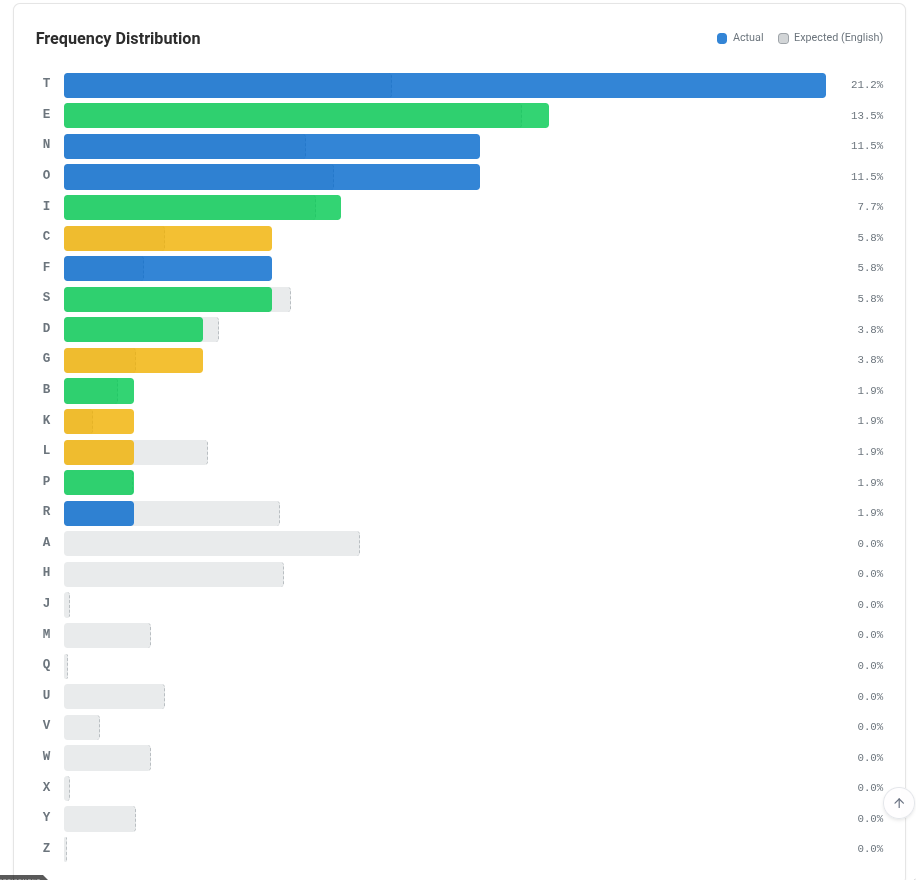
\includegraphics[width=\linewidth]{cipher6_g5_frequency.png}

        \smallskip
        Group 5
    \end{center}

    \begin{center}
        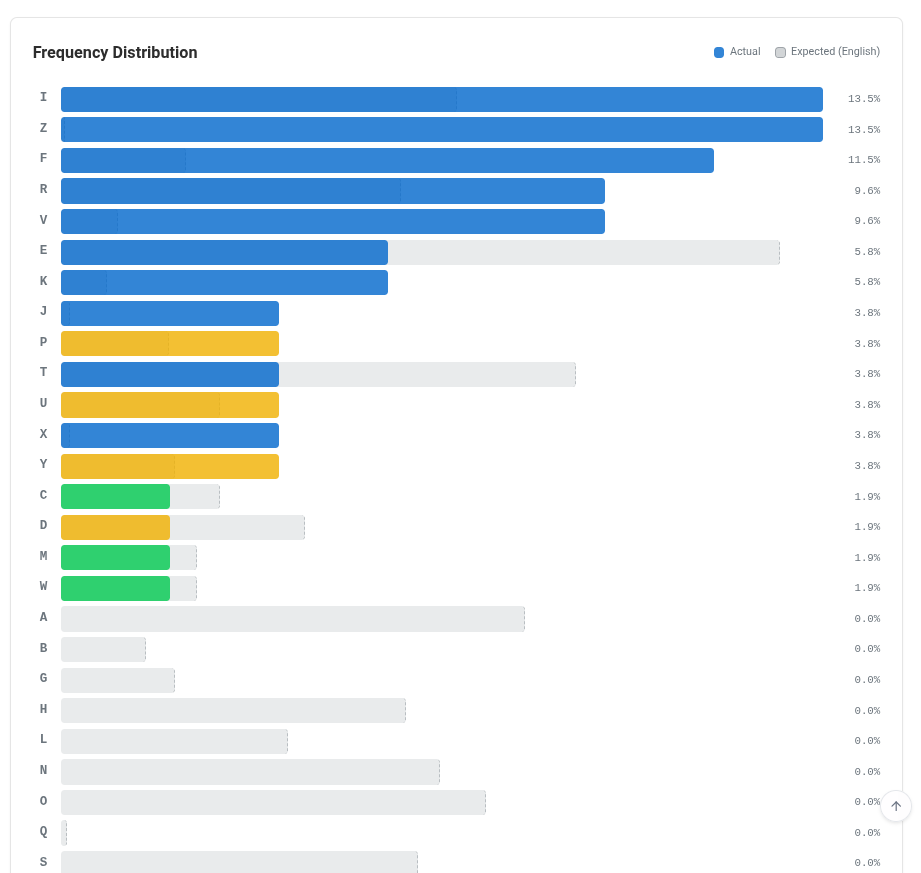
\includegraphics[width=\linewidth]{cipher6_g6_frequency.png}

        \smallskip
        Group 6
    \end{center}

    Same test as the Caesar line. Each row guesses that E is the next tallest bar, then fills in T, A, O, I, N with the same \(x\). A red cell is 0\%, so that row is rejected. The key letter is A shifted by the \(x\) that survives.

    \textbf{Group 1.} C is tried first and sends O to M. U, the other 13.5\% bar, keeps E through N high. Shift 16, key letter Q.

    \begin{center}
    \resizebox{\linewidth}{!}{%
    \begin{tabular}{l c c c c c c c}
    \hline
    Image of E & \(x\) & E & T & A & O & I & N \\
    \hline
    C (13.5\%) & 24 & C 13.5\% & R 1.9\% & Y 3.8\% & \textcolor{red}{M 0.0\%} & G 0.0\% & L 0.0\% \\
    U (13.5\%) & 16 & U 13.5\% & J 9.6\% & Q 11.5\% & E 5.8\% & Y 3.8\% & D 9.6\% \\
    \hline
    \end{tabular}}
    \end{center}

    \textbf{Group 2.} N, C, and U each hit a red cell. Y does not. Shift 20, key letter U.

    \begin{center}
    \resizebox{\linewidth}{!}{%
    \begin{tabular}{l c c c c c c c}
    \hline
    Image of E & \(x\) & E & T & A & O & I & N \\
    \hline
    N (11.5\%) & 9 & N 11.5\% & C 9.6\% & J 3.8\% & X 3.8\% & \textcolor{red}{R 0.0\%} & W 5.8\% \\
    C (9.6\%) & 24 & C 9.6\% & \textcolor{red}{R 0.0\%} & Y 9.6\% & M 3.8\% & G 3.8\% & L 1.9\% \\
    U (9.6\%) & 16 & U 9.6\% & J 3.8\% & Q 1.9\% & \textcolor{red}{E 0.0\%} & Y 9.6\% & D 0.0\% \\
    Y (9.6\%) & 20 & Y 9.6\% & N 11.5\% & U 9.6\% & I 7.7\% & C 9.6\% & H 7.7\% \\
    \hline
    \end{tabular}}
    \end{center}

    \textbf{Group 3.} The first bar is already E, and \(x=0\) keeps every common letter off 0\%. Shift 0, key letter A.

    \begin{center}
    \resizebox{\linewidth}{!}{%
    \begin{tabular}{l c c c c c c c}
    \hline
    Image of E & \(x\) & E & T & A & O & I & N \\
    \hline
    E (19.2\%) & 0 & E 19.2\% & T 5.8\% & A 5.8\% & O 11.5\% & I 7.7\% & N 11.5\% \\
    \hline
    \end{tabular}}
    \end{center}

    \textbf{Group 4.} K, F, A, and L each hit a red cell. W keeps E through N high. Shift 18, key letter S.

    \begin{center}
    \resizebox{\linewidth}{!}{%
    \begin{tabular}{l c c c c c c c}
    \hline
    Image of E & \(x\) & E & T & A & O & I & N \\
    \hline
    K (13.5\%) & 6 & K 13.5\% & \textcolor{red}{Z 0.0\%} & G 3.8\% & U 1.9\% & O 1.9\% & T 3.8\% \\
    F (11.5\%) & 1 & F 11.5\% & U 1.9\% & \textcolor{red}{B 0.0\%} & P 0.0\% & J 5.8\% & O 1.9\% \\
    A (7.7\%) & 22 & A 7.7\% & \textcolor{red}{P 0.0\%} & W 7.7\% & K 13.5\% & E 1.9\% & J 5.8\% \\
    L (7.7\%) & 7 & L 7.7\% & A 7.7\% & H 1.9\% & V 1.9\% & \textcolor{red}{P 0.0\%} & U 1.9\% \\
    W (7.7\%) & 18 & W 7.7\% & L 7.7\% & S 5.8\% & G 3.8\% & A 7.7\% & F 11.5\% \\
    \hline
    \end{tabular}}
    \end{center}

    \textbf{Group 5.} T, the tallest bar, sends I to X, so \(x=15\) is rejected. The next bar is E itself, which gives \(x=0\). A is 0\% here, marked possible: these 52 letters can simply contain no A. T, O, I, and N sit on tall bars and are already those English letters. The shift is confirmed when the other five groups are fixed: subtracting 0 here makes the six groups read as English beginning MAGNETON. The key letter is A.

    \begin{center}
    \resizebox{\linewidth}{!}{%
    \begin{tabular}{l c c c c c c c}
    \hline
    Image of E & \(x\) & E & T & A & O & I & N \\
    \hline
    T (21.2\%) & 15 & T 21.2\% & I 7.7\% & P 1.9\% & D 3.8\% & \textcolor{red}{X 0.0\%} & C 5.8\% \\
    E (13.5\%) & 0 & E 13.5\% & T 21.2\% & A 0.0\% (possible) & O 11.5\% & I 7.7\% & N 11.5\% \\
    \hline
    \end{tabular}}
    \end{center}

    \textbf{Group 6.} I, Z, F, and R each hit a red cell. V keeps E through N high. Shift 17, key letter R.

    \begin{center}
    \resizebox{\linewidth}{!}{%
    \begin{tabular}{l c c c c c c c}
    \hline
    Image of E & \(x\) & E & T & A & O & I & N \\
    \hline
    I (13.5\%) & 4 & I 13.5\% & X 3.8\% & E 5.8\% & \textcolor{red}{S 0.0\%} & M 1.9\% & R 9.6\% \\
    Z (13.5\%) & 21 & Z 13.5\% & \textcolor{red}{O 0.0\%} & V 9.6\% & J 3.8\% & D 1.9\% & I 13.5\% \\
    F (11.5\%) & 1 & F 11.5\% & U 3.8\% & \textcolor{red}{B 0.0\%} & P 3.8\% & J 3.8\% & O 0.0\% \\
    R (9.6\%) & 13 & R 9.6\% & \textcolor{red}{G 0.0\%} & N 0.0\% & B 0.0\% & V 9.6\% & A 0.0\% \\
    V (9.6\%) & 17 & V 9.6\% & K 5.8\% & R 9.6\% & F 11.5\% & Z 13.5\% & E 5.8\% \\
    \hline
    \end{tabular}}
    \end{center}

    The six shifts are 16, 20, 0, 18, 0, 17, so the key is QUASAR. Subtract that repeating shift. The plaintext begins with MAGNETON.

    \smallskip
    {\scriptsize\ttfamily\seqsplit{MAGNETONEMBODIESCOLLABORATIONANDSYNERGYFORMEDFROMMULTIPLEUNITSITDEMONSTRATESTHEPOWEROFCOORDINATIONMAGNETONTEACHESTHATTEAMWORKAMPLIFIESCAPABILITYITREFLECTSTHEIMPORTANCEOFCOLLECTIVEEFFORTANDALIGNMENTSHOWINGTHATCOMBINEDFOCUSSTRENGTHENSINFLUENCEANDEFFECTIVENESSMAGNETONEMBODIESUNITYEFFICIENCYANDSTRATEGICCOORDINATION}}

    \bigskip
    \textbf{Playfair:} Charizard

    \textbf{Explanation:}
    Line 1 is the Playfair ciphertext. The key is a \(5\times 5\) matrix, a permutation of \texttt{A}--\texttt{Z} with \texttt{J} removed, so the key space has size \(25!\approx 1.55\times 10^{25}\). Trying every matrix is not practical. The search used here is simulated annealing (\mbox{\url{https://en.wikipedia.org/wiki/Simulated_annealing}}). The program is available at \href{https://github.com/LyuLucas1207/Classical-Cryptanalysis/tree/main/playfair}{https://github.com/LyuLucas1207/\allowbreak{}Classical-Cryptanalysis/tree/main/playfair}.

    Each candidate key decrypts the ciphertext. The resulting string is scored with English quadgram statistics from \texttt{english\_quadgrams.txt}. That file has one quadgram and its count on each line, for example \texttt{TION 13168375}. A quadgram is four consecutive letters. The score of one quadgram is the base-10 log of its share of the file:
    \[
    S(q)=\log_{10}\!\left(\frac{\mathrm{Count}(q)}{\mathrm{Total}}\right).
    \]
    The numbers below are only an illustration. Suppose the file contained just these rows and the counts summed to \(1{,}000{,}000\):

    \begin{center}
    \begin{tabular}{lr}
    \hline
    Quadgram & Count \\
    \hline
    \texttt{THER} & 100{,}000 \\
    \texttt{HERE} & 50{,}000 \\
    \texttt{XQZB} & 1 \\
    \hline
    \end{tabular}
    \end{center}

    \begin{align*}
    S(\texttt{THER})&=\log_{10}(100{,}000/1{,}000{,}000)=\log_{10}(0.1)=-1,\\
    S(\texttt{HERE})&=\log_{10}(50{,}000/1{,}000{,}000)=\log_{10}(0.05)\approx -1.301,\\
    S(\texttt{XQZB})&=\log_{10}(1/1{,}000{,}000)=-6.
    \end{align*}

    \texttt{THER} is common English, so its score is closer to zero. \texttt{XQZB} is rare, so its score is much lower. The real file is used in the same way. For a candidate plaintext \(P\) of length \(n\), the program adds the score of every four-letter block:
    \[
    S(P)=\sum_{i=1}^{n-3}\log_{10}\Pr(P_i P_{i+1} P_{i+2} P_{i+3}).
    \]
    A block that is missing from the file gets a fixed penalty, \(\log_{10}(0.01/\mathrm{Total})\), about \(-11.6\) for this file. Every term is negative because each probability is below 1, so the total is negative. A larger total, closer to zero, means the decryption looks more like English. On this 300-letter ciphertext, gibberish scores near \(-1800\) and the correct English scores near \(-1336\).

    Simulated annealing searches for a key with a high score. One run starts from a random \(5\times 5\) matrix, or from the alphabetical matrix on the first run. It then proposes a new key by a random edit: with probability \(90\%\) it swaps two letters, with probability \(4\%\) it swaps two rows, with probability \(4\%\) it swaps two columns, and with probability \(2\%\) it shuffles four letters. The new key is decrypted and scored. A higher score is always kept. A lower score is kept with probability
    \[
    \Pr(\text{accept})=\exp\!\left(\frac{S_{\mathrm{new}}-S_{\mathrm{old}}}{T}\right),
    \]
    where \(T\) is the temperature. \(T\) starts at 12 and drops by \(0.5\) after every \(2500\) edits, down to 0. Early on, a worse key is sometimes accepted, so the search can leave a poor matrix. Later it mostly keeps improvements. The code repeats this from a new starting matrix up to 12 times and stops when a score rises above \(-1500\). That cutoff sits between gibberish and readable English. One successful run is enough. The run in the figure reached the best score on attempt 4 of 12, after about one minute.

    \begin{center}
        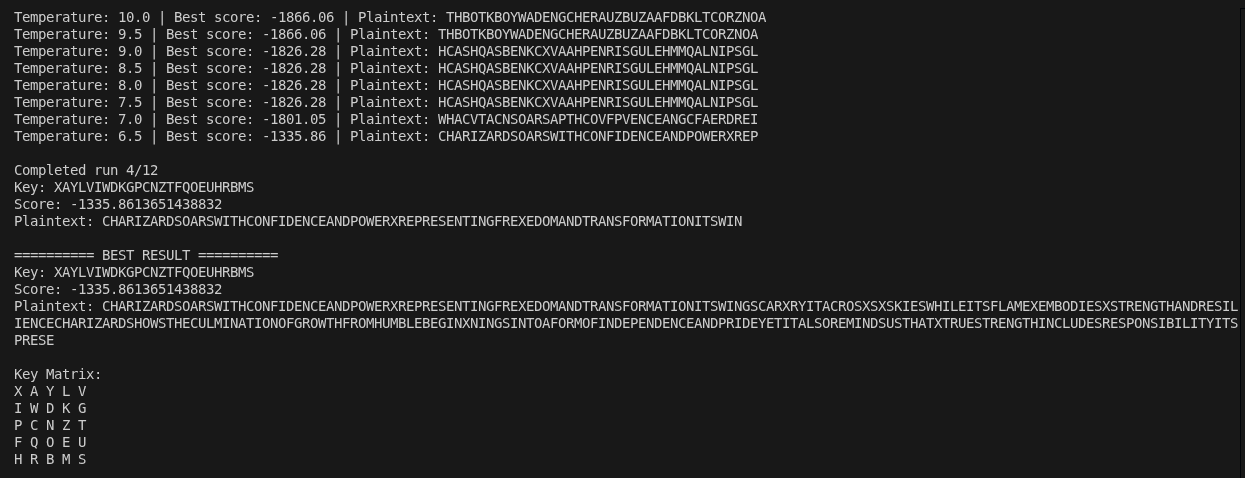
\includegraphics[width=\linewidth]{Playfair.png}
    \end{center}

    The best score is \(-1335.86\). The key, written row by row, is \texttt{XAYLVIWDKGPCNZTFQOEUHRBMS}:

    \begin{center}
    \begin{tabular}{ccccc}
    X & A & Y & L & V \\
    I & W & D & K & G \\
    P & C & N & Z & T \\
    F & Q & O & E & U \\
    H & R & B & M & S \\
    \end{tabular}
    \end{center}

    The decryption begins \texttt{CHARIZARDSOARS}. The \texttt{X}s are the fillers Playfair inserts between doubled letters, such as \texttt{FREXEDOM} for FREEDOM and \texttt{BEGINXNINGS} for BEGINNINGS. Removing those fillers gives the description of Charizard. Encrypting this plaintext with the same matrix returns line 1.

    \smallskip
    {\scriptsize\ttfamily\seqsplit{CHARIZARDSOARSWITHCONFIDENCEANDPOWERXREPRESENTINGFREXEDOMANDTRANSFORMATIONITSWINGSCARXRYITACROSXSXSKIESWHILEITSFLAMEXEMBODIESXSTRENGTHANDRESILIENCECHARIZARDSHOWSTHECULMINATIONOFGROWTHFROMHUMBLEBEGINXNINGSINTOAFORMOFINDEPENDENCEANDPRIDEYETITALSOREMINDSUSTHATXTRUESTRENGTHINCLUDESRESPONSIBILITYITSPRESE}}

    \medskip
    The same plaintext can be checked with a Playfair Analyzer search. That run was allowed to test \(400{,}000{,}000\) keys, the limit set in the tool, out of the \(1.55\times 10^{25}\) possible matrices. It finished in 20 minutes 21 seconds and decrypted the ciphertext to the same Charizard text. Its reported key, \texttt{MSHRBLVXAYKGIWDZTPCNEUFQO}, is the matrix above shifted by whole rows and whole columns. That shift does not change Playfair encryption, so the two keys are the same square.

    \begin{center}
        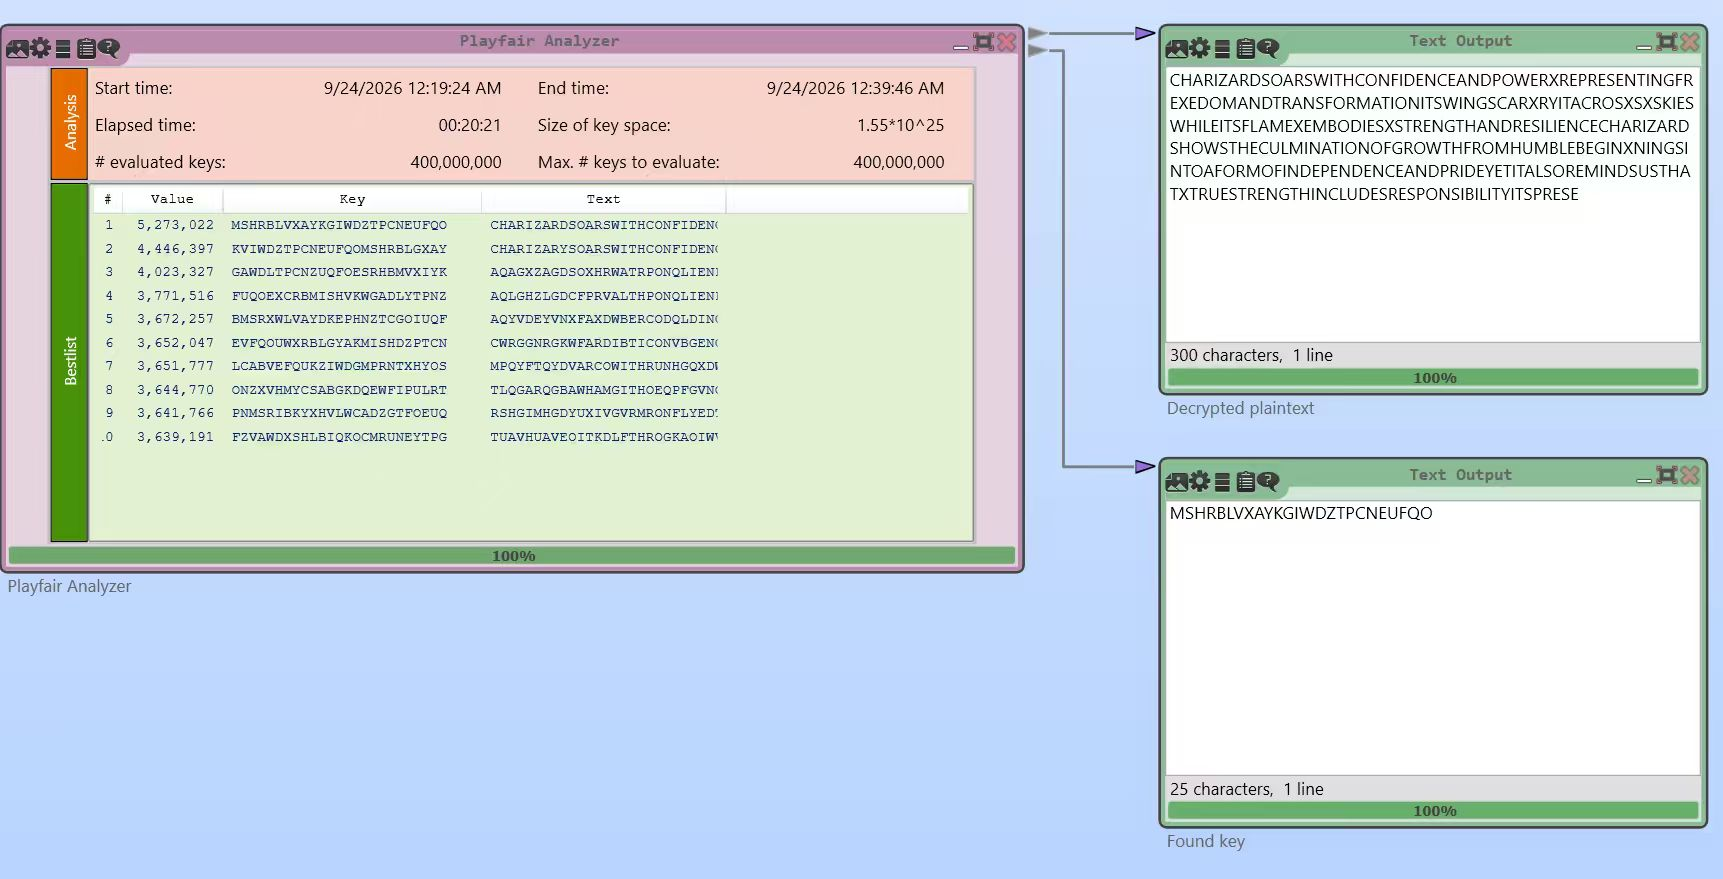
\includegraphics[width=\linewidth]{Playfair_Brute.jpg}
    \end{center}

    \bigskip
    \textbf{OTP (first line):} line 3, Growlithe

    \textbf{Explanation:}
    Lines 3 and 4 use the same OTP key. Each character is one RFC 4648 Base32 symbol, A--Z then 2--7, and each symbol is 5 bits. XORing the two ciphertexts cancels the key, so the result is the XOR of the two plaintexts, not a plaintext letter by itself.

    Line 3 starts with B (\(00001\)) and line 4 starts with F (\(00101\)):
    \[
    00001 \oplus 00101 = 00100,
    \]
    which is E. Line 3 has 310 symbols and line 4 has 273, so the XOR covers the first 273 symbols. It begins EFPYGMCD.

    \smallskip
    {\scriptsize\ttfamily\seqsplit{EFPYGMCDLAA5VJBWCXDZKNE2TVCJDPNQ5OVMYFTMSSAMLBAVNIAZLIAFNVM3VPAS7WAAA4A7Q2TRE6WBT52OWG45LSFDGJ7FM4BAACNPQPBWMCWMXKRTB56VHWTCKHRXSOAKJNJ2ANVAGPSKB6IKIMMDJSXGCBHCQRAFRVVBHMPQAW4HWAVGNQCEXIGITXFI4O3RWWKMKG6MTVQFLYCPUYRORUPPBE3TKAALLJLWRTF77MWMEASEKX5XAWFUADLTKWGLDTMVXXYVG6UAA}}

    \medskip
    RFC 4648 Base32 uses A--Z and 2--7. The value is the position in that list, written as 5 bits.

    \begin{center}
    \scriptsize
    \setlength{\tabcolsep}{4pt}
    \begin{tabular}{c r c c r c}
    \hline
    Char & Value & Bits & Char & Value & Bits \\
    \hline
    A & 0 & 00000 & Q & 16 & 10000 \\
    B & 1 & 00001 & R & 17 & 10001 \\
    C & 2 & 00010 & S & 18 & 10010 \\
    D & 3 & 00011 & T & 19 & 10011 \\
    E & 4 & 00100 & U & 20 & 10100 \\
    F & 5 & 00101 & V & 21 & 10101 \\
    G & 6 & 00110 & W & 22 & 10110 \\
    H & 7 & 00111 & X & 23 & 10111 \\
    I & 8 & 01000 & Y & 24 & 11000 \\
    J & 9 & 01001 & Z & 25 & 11001 \\
    K & 10 & 01010 & 2 & 26 & 11010 \\
    L & 11 & 01011 & 3 & 27 & 11011 \\
    M & 12 & 01100 & 4 & 28 & 11100 \\
    N & 13 & 01101 & 5 & 29 & 11101 \\
    O & 14 & 01110 & 6 & 30 & 11110 \\
    P & 15 & 01111 & 7 & 31 & 11111 \\
    \hline
    \end{tabular}
    \end{center}

    The plaintext uses only A--Z, so a pair that contains 2--7 is impossible. Each remaining pair can be read in either order. The first three XOR symbols are E, F, and P.

    \textbf{E} $=00100$. Twelve letter pairs. Dropped: Y$\leftrightarrow$4, Z$\leftrightarrow$5, 2$\leftrightarrow$6, 3$\leftrightarrow$7.

    \begin{center}
    \small
    \begin{tabular}{c c c c}
    \hline
    First & Bits & Second & Bits \\
    \hline
    A & 00000 & E & 00100 \\
    B & 00001 & F & 00101 \\
    C & 00010 & G & 00110 \\
    D & 00011 & H & 00111 \\
    I & 01000 & M & 01100 \\
    J & 01001 & N & 01101 \\
    K & 01010 & O & 01110 \\
    L & 01011 & P & 01111 \\
    Q & 10000 & U & 10100 \\
    R & 10001 & V & 10101 \\
    S & 10010 & W & 10110 \\
    T & 10011 & X & 10111 \\
    \hline
    \end{tabular}
    \end{center}

    \textbf{F} $=00101$. Twelve letter pairs. Dropped: Y$\leftrightarrow$5, Z$\leftrightarrow$4, 2$\leftrightarrow$7, 3$\leftrightarrow$6.

    \begin{center}
    \small
    \begin{tabular}{c c c c}
    \hline
    First & Bits & Second & Bits \\
    \hline
    A & 00000 & F & 00101 \\
    B & 00001 & E & 00100 \\
    C & 00010 & H & 00111 \\
    D & 00011 & G & 00110 \\
    I & 01000 & N & 01101 \\
    J & 01001 & M & 01100 \\
    K & 01010 & P & 01111 \\
    L & 01011 & O & 01110 \\
    Q & 10000 & V & 10101 \\
    R & 10001 & U & 10100 \\
    S & 10010 & X & 10111 \\
    T & 10011 & W & 10110 \\
    \hline
    \end{tabular}
    \end{center}

    \textbf{P} $=01111$. Ten letter pairs. Dropped: Q$\leftrightarrow$7, R$\leftrightarrow$6, S$\leftrightarrow$5, T$\leftrightarrow$4, U$\leftrightarrow$3, V$\leftrightarrow$2.

    \begin{center}
    \small
    \begin{tabular}{c c c c}
    \hline
    First & Bits & Second & Bits \\
    \hline
    A & 00000 & P & 01111 \\
    B & 00001 & O & 01110 \\
    C & 00010 & N & 01101 \\
    D & 00011 & M & 01100 \\
    E & 00100 & L & 01011 \\
    F & 00101 & K & 01010 \\
    G & 00110 & J & 01001 \\
    H & 00111 & I & 01000 \\
    W & 10110 & Z & 11001 \\
    X & 10111 & Y & 11000 \\
    \hline
    \end{tabular}
    \end{center}

    These pairs were matched against the names of the first 151 Pok{\'e}mon. The first four XOR symbols, EFPY, leave one pair of names: Growlithe and Cubone. The next two symbols agree as well. G$\oplus$C, R$\oplus$U, O$\oplus$B, W$\oplus$O, L$\oplus$N, and I$\oplus$E are E, F, P, Y, G, and M.

    \begin{center}
    \small
    \begin{tabular}{c c c c}
    \hline
    Position & Growlithe & Cubone & XOR \\
    \hline
    1 & G & C & E \\
    2 & R & U & F \\
    3 & O & B & P \\
    4 & W & O & Y \\
    5 & L & N & G \\
    6 & I & E & M \\
    \hline
    \end{tabular}
    \end{center}

    Taking the two openings GROWLITHEREPRESENTS and CUBONEREPRESENTS, the XOR of the shared length is still the ciphertext XOR. Line 3 is assigned to Growlithe and line 4 to Cubone.

    \bigskip
    \textbf{OTP (second line):} line 4, Cubone

    \textbf{Explanation:}
    Cubone. This line is the full 273-symbol ciphertext used in the XOR.
\end{answer}

% Include this section only if you used generative AI.
% It must be between half a page and one page long, and cannot be written by AI.
\begin{samepage}
\section*{Generative AI Disclosure}

We used a generative AI coding assistant for the Playfair program in Question 3. I told the assistant the simulated annealing logic and gave it a basic version of the code: start from a key matrix, decrypt the ciphertext, score it with English quadgram frequencies, then swap two letters or, less often, two rows or two columns. A higher score is kept, and a lower score is sometimes kept as the temperature decreases. The assistant implemented the program from that logic and that basic code. The code is at \href{https://github.com/LyuLucas1207/Classical-Cryptanalysis/tree/main/playfair}{https://github.com/LyuLucas1207/\allowbreak{}Classical-Cryptanalysis/tree/main/playfair}. I ran it and checked that the plaintext is Charizard.
\end{samepage}

\end{document}
